% !TEX encoding = UTF-8 Unicode
%%==================================================
%% thanks.tex for SJTU Bachelor Thesis
%% version: 0.5.2
%% Encoding: UTF-8
%%==================================================

\chapter{Stock Return Series Prediction System}
\label{chap:system}

This chapter explains in details about the composition of 
the stock return series prediction system and functionality of each module.
Sec.\,\ref{sec:system:overview} firstly present an overview of the system,
introducing the entire data flow and module connection.
Then, in Sec.\,\ref{sec:system:function}, structure of each part is analyzed,
including its intention, input and output, and settings specific to this thesis.
Sec.\,\ref{sec:system:improvement} focuses on some of these settings 
and proposes several ideas concerning potential for improvement.
The full version of the system realization with Python programming is appended to the thesis 
in Appendix \ref{app:code}.

%%%%%%%%%%%%%%%%%%%%%%%%%%

\section{Overview}
\label{sec:system:overview}

		\begin{figure}[!hbt]
        \center
        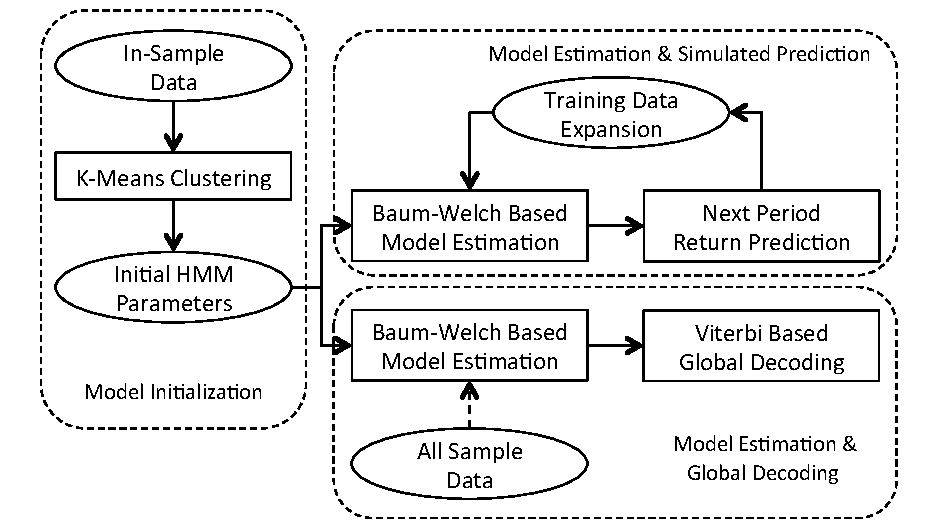
\includegraphics[width=\textwidth]{system.pdf}
        \caption{Overview of the stock return series prediction system}
        \label{fig:system:overview}
        \end{figure}
The stock return series prediction system is composed of two major parts,
model initialization, and simulated prediction; 
the latter part can be further split into two sub-parts, 
model estimation with Baum-Welch (EM) algorithm and prediction based on the model.
Apart from these two major parts, 
a global decoding module is also included in the system 
with purpose to conducted analysis of sample data within the entire observation period.

Illus.\,\ref{fig:system:overview} is a brief overview of the system.
The organization of the system are constructed and will be explained accordingly as follows
	\begin{itemize}
	\item \textbf{Model initialization,} including data pre-processing,
		  initial guesses for parameters based on K-Means clustering.
	\item \textbf{Simulated prediction,} including two sub-parts:
		  \begin{enumerate}
		  \item \textbf{EM based model estimation,} i.e.\,estimation of the state transition matrix
		  		and conditional distribution parameters with EM algorithm.
		  \item \textbf{Prediction,} for stock return of the next period based on 
		  		aforementioned model estimation results.
		  \end{enumerate}
	\item \textbf{Global decoding,} including model estimation and 
		  decoding based on Viterbi algorithm. 
		  The model in this part takes in all sample data in order to 
		  provide analysis of the entire period and the most likely sequence of hidden states.
	\item \textbf{Results saving and visualization.} This part is significant to the system in practice,
		  but needless to be explained in details. 
		  All numerical results are exported in the form of \texttt{.csv} files and 
		  visualizations are carried out on the results.
	\end{itemize}

%%%%%%%%%%%%%%%%%%%%%%%%%%

\section{System composition and functionality}
\label{sec:system:function}
This section is focused on detailed descriptions of 
each part listed above in Sed. \ref{sec:system:overview}.
The part of results saving and visualization is, however, omitted in this section
since the process is more about convenience and intuition 
while it has very little to do with the system itself.


\subsection{Model initialization}
\label{sec:system:function:init}
The data pre-processing work include data downloading and tidying.
A complete input data file consists of two columns, 
the first standing for the timeline and the second for the observed closing prices.
Timeline should be uniformed for each trading day (or trading year in daily cases),
and thus missing value of closing prices should be filled.
Here we fill the missing ones with previous values,
but it is not the only method and sometimes 
linear interpolation or even spline interpolation are implemented for data filling
(e.g.\,see \cite{Beckers:2003do,Reuter:2007cv}).

In order to construct a K-Means model, 
further adjustment and transformation should be made on the raw data.
Firstly we calculate the log return series out of the price series,
and then estimate the standard deviation on each observing time node
through calculating the rolling historical standard errors,
as is shown in Eq.\,\ref{eq:system:data}
		\begin{equation}
		\label{eq:system:data}
		\begin{aligned}
		\text{log return}: r_t & = ln\big( \frac{P_{t}}{P_{t-1}} \big),\ t = 1,2,\dots, \\
		\text{standard deviation}: \sigma_t & = 
			\sqrt{\frac{1}{nf - 1}\sum_{i=t-nf+1}^{nf} (r_i - \bar{r})^2},\ t \geq nf.
		\end{aligned}
		\end{equation}
where $n$ is the number of rolling days and $f$ represents the number of data within each trading day.
For data with different observation frequency, 
$f$ vary (e.g.\,$f=1$ for daily data and $f=24$ for 10min data) but we keep $n$ the same;
more specifically, we choose $n=5$ in this system.

		\begin{figure}[!hbt]
        \center
        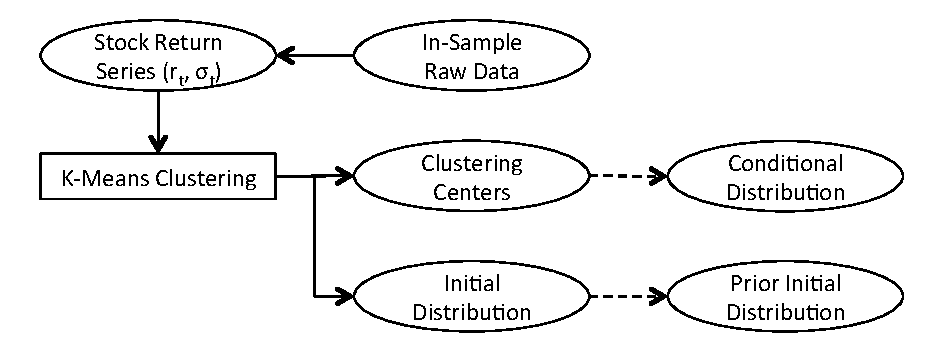
\includegraphics[width=\textwidth]{initialization.pdf}
        \caption{Model initialization module}
        \label{fig:system:init}
        \end{figure}
Now K-Means model takes in a two dimensional time series,
i.e.\,the stock return series and 5-day historical standard deviation series.
Given the number of states, $k$, 
the model generates $k$ clustering centers and corresponding probability distribution,
which are then taken as initial guesses for HMM conditional distribution parameters 
and initial state distribution separately.
Initial guesses for each entry of the transition matrix is arbitrarily set as equal.
The process follows the steps in Illus.\,\ref{fig:system:init}

Notice that K-Means is a very common method to 
find the prior distribution of the parameters \cite{Brailovskiy:2014wu},
while there are also some other methods to find the prior,
e.g.\,generating random vector satisfying the numerical constraints \cite{Hassan:2005uw},
or introduction of machine learning techniques like artificial neural networks (ANN) 
and genetic algorithms (GA) \cite{Hassan:2007hk}. 


\subsection{Simulated prediction}
\label{sec:system:function:prediction}
Simulated prediction module processes with a time loop, 
containing two parts within each loop, model estimation and prediction.
Every time a loop is finished,
we incorporate the real historical return of the next period into the training data set
and process the time horizon to the next period,
estimate the model with the new data set in order to 
predict the return of one more next period.
The iterations is visually described in Illus.\,\ref{fig:system:overview}.


\subsubsection{EM based model estimation}
\label{sec:system:function:prediction:EM}

		\begin{figure}[!hbt]
	    \center
	    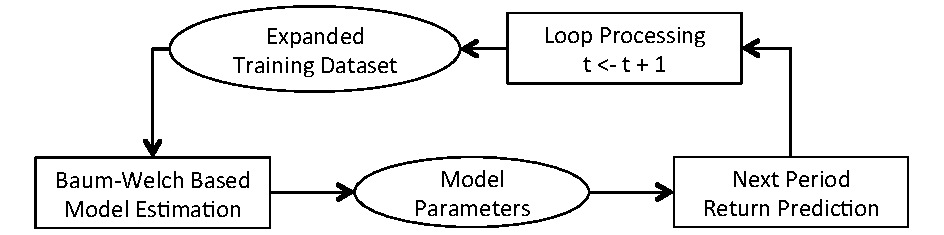
\includegraphics[width=\textwidth]{EM.pdf}
	    \caption{EM based model estimation procedure}
	    \label{fig:system:EM}
	    \end{figure}
Model estimation refers to find the estimations of model parameters, 
including state transition matrix parameters (each entry of the matrix) and
conditional distribution parameters 
(probability density distributions of observed variables conditional on each state).
The method is fully explained in Sec.\,\ref{sec:HMM:EM} 
so we avoid the unnecessary repetition here.
Visual description of the procedure is shown in Illus.\,\ref{fig:system:EM}.

There is something though should be cleared.
As we mentioned before, 
initial guesses for model parameters of the very first loop is found 
with K-Means clustering based on in-sample data.
We use the same initial guesses for all of the following loops,
i.e.\,initialization is carried out only once and 
we no more perform K-Means on the expanded training dataset.
Besides, using the same initial guesses also means that 
the EM algorithm starts from the same parameters for different iterations.
Another way to improve the initial guesses is to 
use the estimation results from the previous loop as the initial guess for the next one,
which shall largely relieve the computational burden and reduce the running time of the system.
However, the change of the training dataset is so small that 
it is reasonable to assume that model parameters change very little.
Thus, it is possible that the initial guess is close enough to the final result 
so that the algorithm prematures due to precision limits,
and that is why the system does not take this way to set the initial guesses.


\subsubsection{Prediction}
\label{sec:system:function:prediction:prediction}
Prediction for the next return is calculated through the estimation results found with EM.
The calculation is simply put as follows:
		\begin{subequations}
		\begin{align}
		\label{eq:system:prediction:ret}
		r_{t+1} & = \bdelta^{\prime} \bGamma \bmu, \\
		\label{eq:system:prediction:std}
		\sigma_{t+1} & = \sqrt{\bdelta^{\prime} \bGamma \bsigma^2},
		\end{align}
		\end{subequations}
where
		\begin{equation}
		\label{eq:system:mu}
		\bmu = (\mu_1, \mu_2, \dots, \mu_N)
		\end{equation}
are expectations of the conditional distributions, and
		\begin{equation}
		\label{eq:system:sigma}
		\bsigma^2 = (\sigma^2_1, \sigma^2_2, \dots, \sigma^2_N)
		\end{equation}
are variances of the conditional distributions,
and $\bdelta$ represents the final distribution of the hidden state 
and $\bGamma$ stands for the state transition matrix.
Notice that an implied assumption of Eq.\,\ref{eq:system:prediction:std} is that
the distributions conditional on hidden states are independent
so the variances are added without covariance terms.
The prediction results are then to be compared with the actual historical returns 
and corresponding standard deviations are used to find the confidence band.

There are two ways to plot the prediction results.
The first one is to fix the price level at the last in-sample date,
of which the stock price is denoted as $P_0$.
We denote the predicted returns as $\hat{r}_i, i = 1,2,\dots,t$,
and thus the prediction result of $\hat{P}_t$ is that
		\begin{equation}
		\hat{P}_t = P_0 e^{\sum_{i=1}^{t}\hat{r}_i}.
		\end{equation}
The second one is called the adaptive prediction, 
which incorporates not only the information of returns but also prices of the data.
In order to predict the price at time $t$, 
we firstly predict the return $\hat{r}_t$ and compute the price given the price at time $t-1$,
that is
		\begin{equation}
		\hat{P}_t = P_{t-1} e^{\hat{r}_t}.
		\end{equation}
In the first kind of prediction, errors of return series predictions accumulate,
so it is very likely that the adaptive prediction performs much better.
We will examine this idea in Ch.\,\ref{chap:positive}.


\subsection{Global decoding}
\label{sec:system:function:decoding}

		\begin{figure}[!hbt]
        \center
        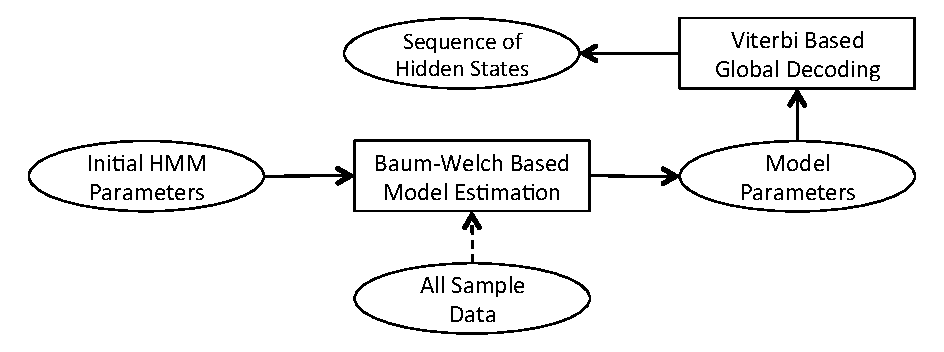
\includegraphics[width=\textwidth]{decoding.pdf}
        \caption{Global decoding module}
        \label{fig:system:decoding}
        \end{figure}
The global decoding module is independent with the simulated prediction module,
and is not the major focus of the prediction system.
The aim of this module is to provide a HMM-based description of 
sample data over the entire observation period.
Traditional methods enable us to know elementary statistics about the data 
(e.g.\,mean, variance, skewness, etc.),
but with Viterbi algorithm we are able to know 
how the hidden states are distributed across the history and 
whether the result matches our conjectures and common senses.

The procedure is illustrated in Illus.\,\ref{fig:system:decoding}.
With initial HMM parameters found in the model initialization module 
(Sec.\,\ref{sec:system:function:init})
we set up the model with all sample data
\footnote{Initial parameters are found with in-sample data instead of all of them. 
Considering the length of out-of-sample data is much shorter than the in-sample,
and the fact that initial guesses do not have large effect on the eventual optimal results,
we choose to remain the initial guesses rather than 
perform another initialization based on all sample data}.
The Viterbi algorithm based decoding is then conducted to 
deduce the most probable sequence of hidden states during the observation period.

%%%%%%%%%%%%%%%%%%%%%%%%%%

\section{Potential for improvement}
\label{sec:system:improvement}
Heretofore the system is complete to perform analysis and predictions 
for the stock return series.
Well functioning as the system is,
it can be further improved and perfected for better performances,
e.g.\,more thorough description of the dataset and more correct and accurate predictions.
We propose several perspectives where potential for improvement may exist.

\subsection{Multiple observed variables}
\label{sec:system:improvement:variable}
Currently the input for the system is a simple observation series on only one variable,
i.e.\,the log return of the stock, derived from its closing price.
However, the information embedded in the single closing price series is so little 
that it cannot capture many of the properties of the stock.
One way to improve the case is to incorporating more observed variables,
e.g.\,opening, low, high and closing prices, 
and to find the conditional observing probability with Gaussian mixture models (GMM)
\cite{Hassan:2005uw,Gupta:2012gm,Brailovskiy:2014wu}.
One of the formulations from \cite{Gupta:2012gm} can be generalized as follows:
		\begin{subequations}
		\begin{align}
		\bo_t & = \big( \frac{\text{close} - \text{open}}{\text{open}},
					  \frac{\text{high} - \text{open}}{\text{open}},
					  \frac{\text{open} - \text{low}}{\text{open}} \big) \\
		b_j(\bo_t) & = \sum_{n = 1}^{N} c_{jn} N(\bo_t,\bmu_{jn},\bsigma_{jn}),
		\end{align}
		\end{subequations}
where $\bo_t$ is the vector of observed variables (observed vector),
$b$ is the observing probability of $\bo_{t}$ conditional on the $j^{th}$ state,
$c$ is the GMM weight and $\bmu, \bsigma$ are GMM parameters.

The idea could be furthered to incorporate more factors apart from the observing prices,
such as financial indicators or economic indicators.
For example, \cite{Wasson:2009dh} presents a way to include Boltzman chain, 
a generalized HMM, into the multi-factor binding genome model.
Including more observed variable may require some other statistical techniques 
since the Gaussian distribution assumption could fail for these variables.
Principal component analysis (PCA) and machine learning theories like neural network (NN)
are commonly implemented methods \cite{Bengio:1992ke,Tipping:1999db,Hassan:2007hk}.


\subsection{Multiseries HMM}
\label{sec:system:improvement:series}
In order to include multiple observed variables, 
the conditional distributions should be accordingly designed and modified.
Another way to make multiple observed variables compact with the original Gaussian distribution
is to introduce the multiseries HMM model,
where the observation is a series of vectors rather than one-dimensional time series.
See \cite{Zucchini:2009df} for more details.


\subsection{Multiple latent variables}
\label{sec:system:improvement:latent}
Apart from improvements from the angle of observed variables,
the latent variable, i.e.\,the hidden states, can also be improved.

The latent variable we use in this thesis is categorical,
which means it merely represents the set of hidden states,
while the states are just labels without realistic statistical meanings.
However, the hidden states can be expressed in other ways that 
they are mathematically meaningful,
and so the latent variable is included in the conditional distribution function of 
the observed variables as a parameter, either discrete or continuous.

For example, time-variation properties are considered for 
the discrete latent variables in \cite{Dias:2015ky};
properties and theories related to continuous latent variables 
are introduced in \cite{Creal:2012ct}.
We will further discuss about the topic in Sec.\,\ref{sec:future:PF}.

Like observed variables, the number of latent variables can be over one
so can the dimension of it, 
and we do not expand the topic here.


